% generated by plots/fig5_spread.py --- do not edit the numbers by hand
% figure* --- the chapter is two-column and this does not fit one
\begin{figure*}[tp]
\centering
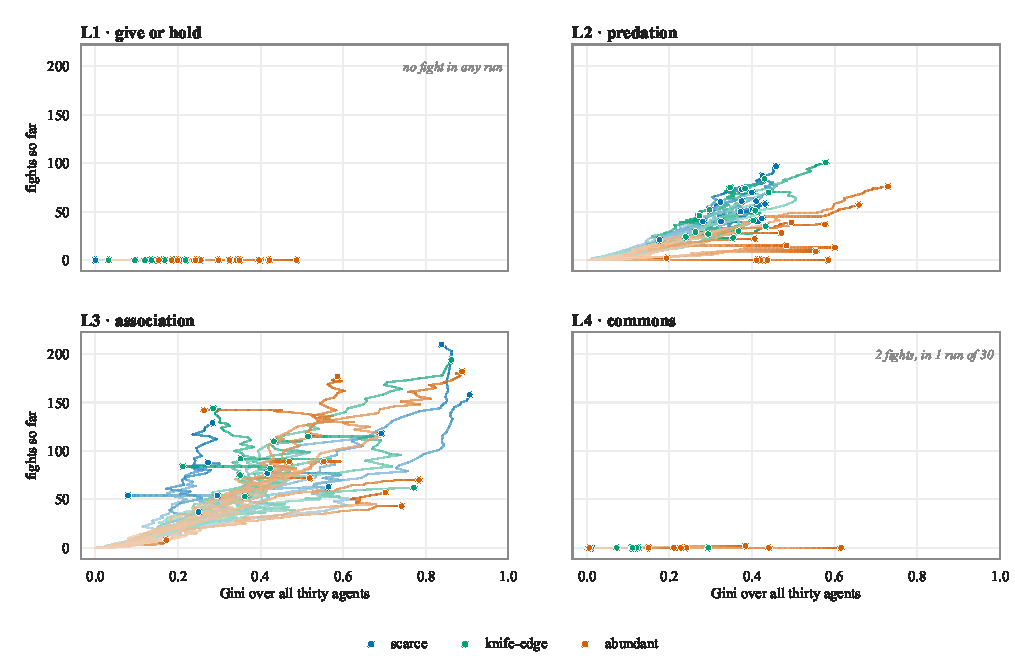
\includegraphics[width=\linewidth]{figures/fig5_spread/spread.pdf}\\[2pt]
\caption[Where a run ends up, and how it got there]{%
\textbf{Where a run ends up, and how it got there.} One line per production run, traced round by round from the opening position to the close, palest at the first round and deepest at the last, with the endpoint marked. Inequality over all thirty agents across the bottom and fights so far up the side, so a line can only climb, and a line that goes flat is a run that has stopped fighting. Every run begins at the origin, since thirty agents each hold a hundred and nothing has been struck. 15 runs per payoff cell at L1 and L2 and 10 at L3 and L4, production model only. The vertical scale is shared, so the two panels whose lines stay on the floor are panels in which nothing was ever struck and not panels with nothing in them.}
\label{fig:spread}
\end{figure*}
